\documentclass[t]{beamer}
\usepackage{beamerthemeSzeged}
\usecolortheme{beaver}
\usepackage{graphicx}
\usepackage{multimedia}
\usepackage{media9}

\title{Impact of Different Hose Stream Applications during Fire Suppression}
\author{Joseph Willi}
\institute [ ] % (optional, but mostly needed)
{\small University of Illinois at Urbana-Champaign\\
 %\includegraphics[scale=.1]{illini.jpg}\\
EL Fire Research Division - Fire Fighting Technology Group}
\date{\small August 6, 2014}

\begin{document}

\setbeamertemplate{itemize items}[circle]
\setbeamercolor{titlelike}{bg=gray!10!white}
\setbeamercolor{frametitle}{bg=gray!10!white}
\setbeamercolor{subsection in head/foot}{bg=black!15!white}
\setbeamercolor{background canvas}{bg=black!15!white}
\setbeamercolor{itemize item}{fg=darkred} % all frames will have red bullets
\beamertemplatenavigationsymbolsempty %removes navigation bar from all slides

\frame[plain]{\titlepage}%Oppurtunity to evaluate the effectiveness of different hose streams on fire suppression

\addtobeamertemplate{navigation symbols}{}{
    \usebeamerfont{footline}
    \usebeamercolor[gray]{footline}
    \hspace{1em}
    \insertframenumber/\inserttotalframenumber
} %adds frame number to slides

\section{Importance of Researching Fireground Tactics}
\begin{frame}[c]
\centerline{\colorbox{gray!15!white}{\color{darkred}\begin{Large}Importance of Researching Fireground Tactics\end{Large}}}
\end{frame}

\begin{frame}
\frametitle{How are Tactics Chosen on the Fireground?}
\begin{columns}
\column{.7\framewidth}
\begin{small}{Decisions based on habits learned from training 
\\~\\
Training based on a set of standard operating procedures (SOPs)
\\~\\
SOPs vary from entity to entity - different people have different opinions
\\~\\
More difficult to rely solely on experience today
\\~\\
Firefighters need to know the science behind tactics
\\~\\
Research bridges the gap between understanding how the fire behaves in its environment and how the fire environment will change when a specific tactic is implemented
}\end{small}
\column{.3\framewidth}
\\~\\
\centerline{\includegraphics[scale=.18]{FIRE.pdf}}
\end{columns}
\end{frame}

%\begin{frame}
%\frametitle{Fireground Tactics Research}
%Covers variety of topics
%\\~\\
%Investigations of close calls and line of duty deaths
%\\~\\
%Full-scale fire experiments to evaluate the effectiveness of certain tactics
%\\~\\
%Provides physical examples that can be related to fire behavior
%\end{frame}
%Forced convection means that the mass flow rate of the adjacent fluid (gas or liquid) is known and its temperature is the result of heat exchange between body and fluid

\begin{frame}
\frametitle{Changing the Flow Path}
Smoke and heat from a fire travel the path of least resistance 
\\~\\
Anyone in the flow path is exposed to hazardous conditions from the increased flow of heat and smoke
\\~\\
Paths can be altered through opening and closing windows and doors in the structure
\\~\\
\begin{columns}
\column{.5\framewidth}
\centerline{\includegraphics[scale=.46]{flow_path.png}}
\column{.5\framewidth}
\centerline{\includegraphics[scale=.46]{fds_flow_path.png}}
\end{columns}
\end{frame}

\section{Hose Streams}
\begin{frame}[c]
\centerline{\colorbox{gray!15!white}{\color{darkred}\begin{Large}Hose Streams\end{Large}}}
\end{frame}

\begin{frame}
\frametitle{What is a Hose Stream?}
\begin{columns}
	\column{.65\framewidth}
Stream of water or extinguishing agent discharged from a hose during fire suppression
\\~\\
Choice of stream dependent upon many factors
\\~\\
Streams vary in numerous ways
\\~\\
Many opinions throughout fire service about the ``best" stream
	\column{.3\framewidth}
	\\~\\
	\centerline{\includegraphics[scale=.17]{Combination_Nozzle.pdf}}
\end{columns}
\end{frame}

\begin{frame}
\frametitle{Different Hose Streams Considered}
\centerline{\movie[height=6.75cm, width=12.8cm, poster,loop,autostart]{}{Hose_Stream_Comparison_Full.avi}}
\end{frame} 

\begin{frame}%talk about GPMs
\frametitle{Different Application Patterns Considered}
\centerline{\movie[height=6.75cm, width=12.8cm,poster,loop,autostart]{}{Application_Pattern_Comparison.avi}}
\end{frame}

\section{Experimental Setup and Results}
\begin{frame}[c]
\centerline{\colorbox{gray!15!white}{\color{darkred}\begin{Large}Experimental Setup and Results\end{Large}}}
\end{frame}

\begin{frame}
\frametitle{Overview of Experiments - Test Structures}
Conducted in two structures located at the Delaware County (DelCo) Emergency Training Services Training Center
%Structures surrounded by 2foot concrete blocks; were Y x Z, serving as a full scale representation of a typical residential structure
	\begin{columns}
    	\column{.5\framewidth}
    	\\~\\
		\centerline{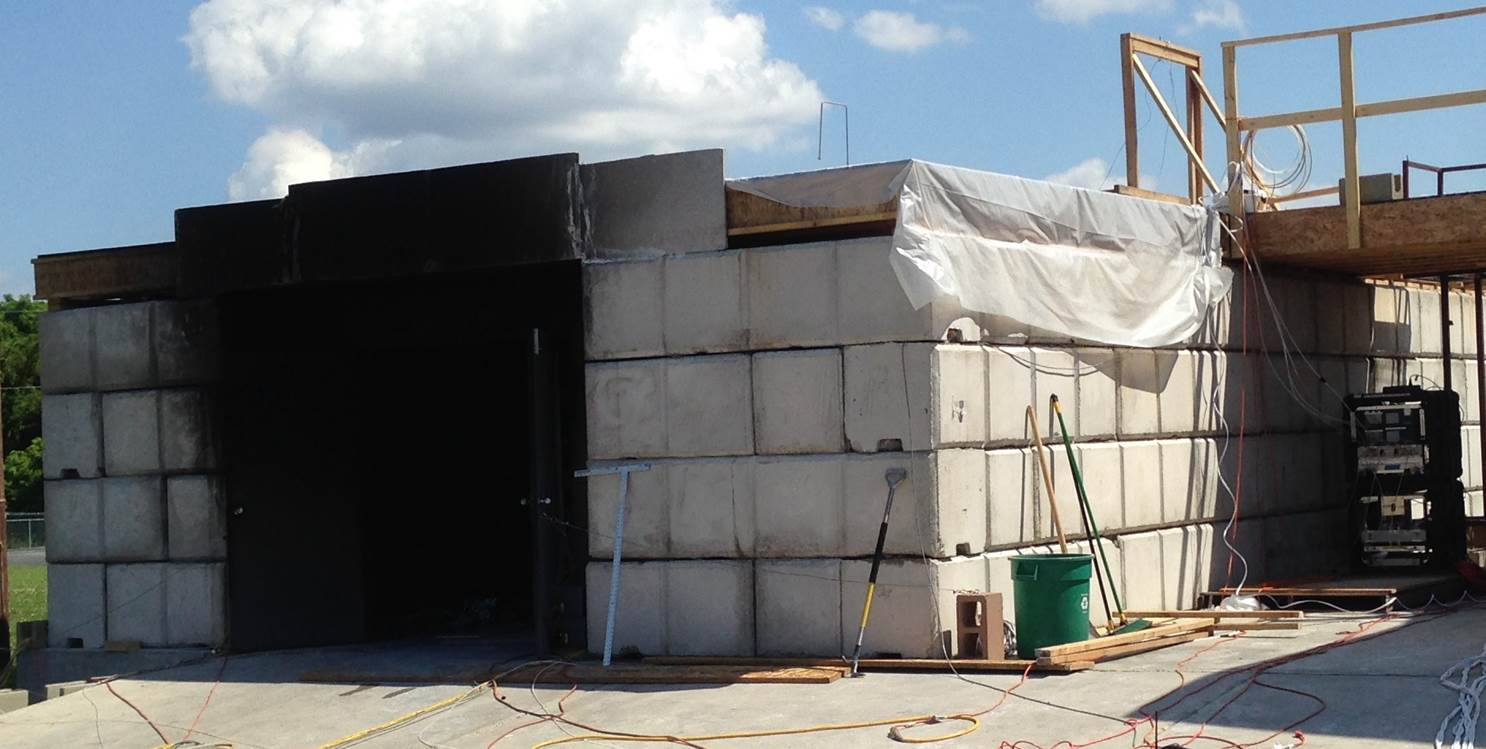
\includegraphics[scale=.245]{east_structure.pdf}}
    	\column{.5\framewidth}
    	\\~\\
		\centerline{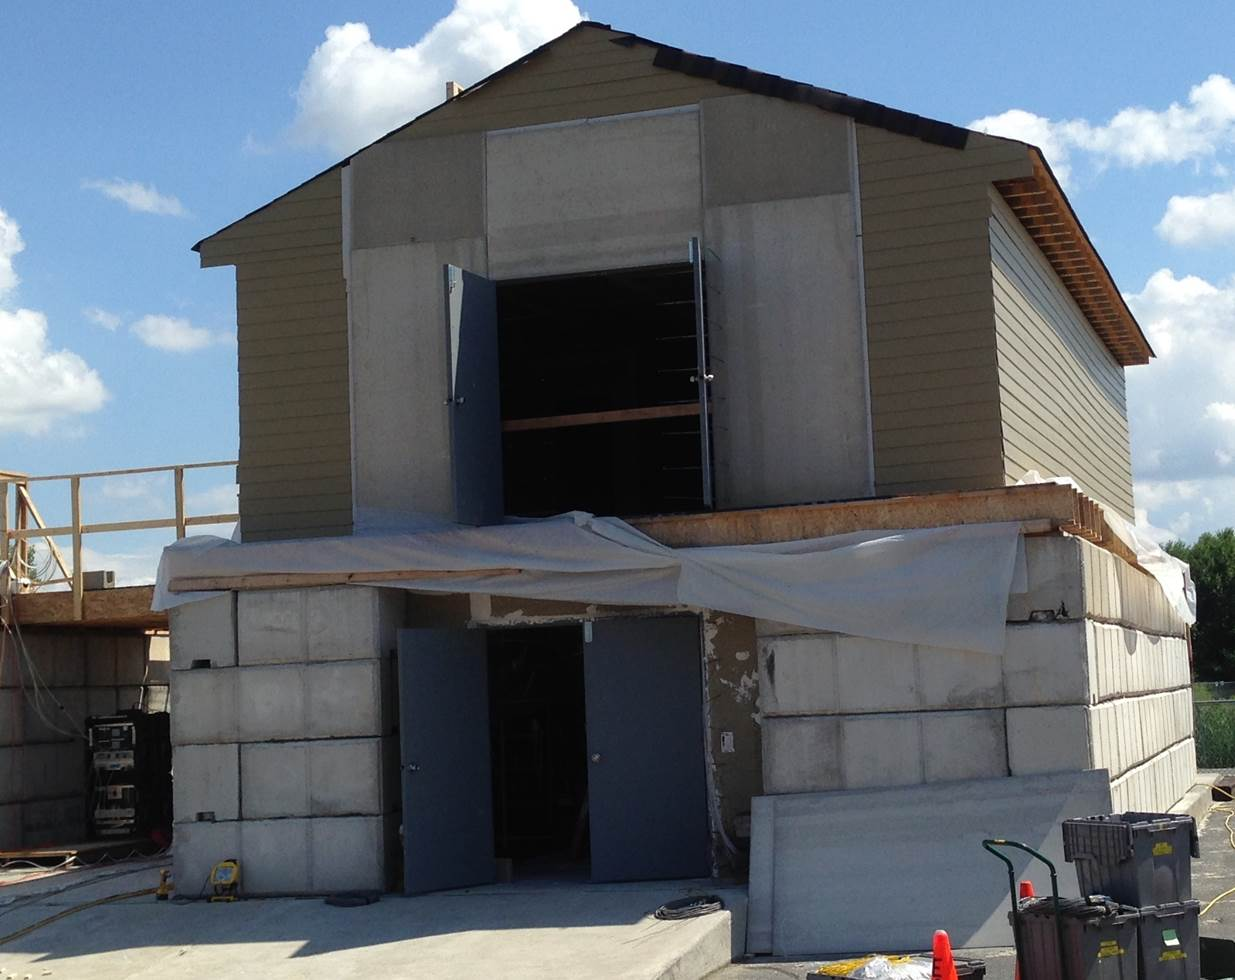
\includegraphics[scale=.245]{west_structure.pdf}}
	\end{columns}
\end{frame}

\begin{frame}
\frametitle{Overview of Experiments - Types of Experiments}
\vspace{\baselineskip}	
\vspace{\baselineskip}
	\begin{columns}%discuss cold flow tests with PPV fan, work on explanation; cold flow tests -> hose tests -> full scale incremental fire tests
		\column{.33\framewidth}
		\centerline{Cold Flow Tests}
		\centerline{\includegraphics[scale=.165]{Cold_Flow_PPV.pdf}}	
		\\~\\ \pause
    	\column{.33\framewidth}
		\centerline{Hose Tests}
		\centerline{\includegraphics[scale=.165]{hose_test.pdf}}
		\\~\\ \pause
		\column{.33\framewidth}
		\centerline{Fire Tests}
		\centerline{\includegraphics[scale=.165]{fire_test.pdf}}
	\end{columns}
\end{frame}

\begin{frame}[c]
\centerline{\colorbox{gray!15!white}{\color{darkred}\begin{Large}Two Story Structure Hose Test\end{Large}}}
	\begin{columns}[T]
		\begin{column}{.5\framewidth}
		\centerline{\includegraphics[scale=.23]{West_Hose_SS.pdf}}
		\end{column}
		\begin{column}{.5\framewidth}
		\centerline{\includegraphics[scale=.23]{West_Hose_WF.pdf}}
		\end{column}
	\end{columns}
\end{frame}

\begin{frame}
\frametitle{Two Story - Hose Test Setup}
\centerline{\includegraphics[width=10cm, height=7cm]{West_Hose_Setup.pdf}}
\end{frame}

\begin{frame}%velocity in m/s vs time in seconds; consists of 8 BDPs evenly spaced in the doorway, starting with the black line at the top in the legend which was right below the door way, all the way to the gold line which is the air flow right above the floor; negative air flow indicates flow in the opposite direction(down the stairwell) and there is little of that from mixing of the air
\frametitle{Two Story - Hose Test Results - Straight Stream}
\centerline{\includegraphics[scale=.44]{West_Hose_SS_BDP10.pdf}}
\end{frame}

\begin{frame}%WF draws in significantly more air due to the larger area of the pattern, it's almost as if it's acting like a fan, drawing the air into the structure
\frametitle{Two Story - Hose Test Results - Wide Fog}
\centerline{\includegraphics[scale=.44]{West_Hose_WF_BDP10.pdf}}
\end{frame}

\begin{frame}[c]
\centerline{\colorbox{gray!15!white}{\color{darkred}\begin{Large}Two Story Structure Fire Test\end{Large}}}
\end{frame}

\begin{frame}
\frametitle{Two Story - Fire Test Setup}
\centerline{\includegraphics[width=10cm, height=7cm]{West_Fire_Setup.pdf}}
\end{frame}

\begin{frame}
\frametitle{Two Story - Fire Test Video}
\centerline{\movie[height=3.25cm, width=10cm,,poster]{}{Fire_Application_SS.avi}}
\centerline{\movie[height=3.25cm, width=10cm,,poster]{}{Fire_Application_WF.avi}}
\end{frame}

\begin{frame}%stress significance of velocity increase and impact they have on flow path
\frametitle{Two Story - Fire Test Results - Stairwell Door}
\centerline{\includegraphics[scale=.45]{West_Fire_SSWF_BDP10.pdf}}
\end{frame}

\begin{frame}%explain plot; mention steady temperatures near floor because that is where low pressure inlet is, describe 
\frametitle{Two Story - Fire Test Results - 2\textsuperscript{nd} Level Rear Door}
\centerline{\includegraphics[scale=.45]{Second_Story_WFSS_TC11.pdf}}
\end{frame}

\begin{frame}[c]
\centerline{\colorbox{gray!15!white}{\color{darkred}\begin{Large}Single Story Structure Fire Test\end{Large}}}
\end{frame}

\begin{frame}
\frametitle{Single Story - Fire Test Setup}
\centerline{\includegraphics[scale=.29]{East_Fire_Setup.jpg}}
\end{frame}

\begin{frame}
\frametitle{Single Story - Fire Test Results - Middle Room}
\centerline{\includegraphics[height=7.25cm,width=10.5cm]{East_Fire_SSNF_TC3.pdf}}
\end{frame}

\begin{frame}
\frametitle{Single Story - Fire Test Results - Front Room}
\centerline{\includegraphics[height=7.25cm, width=10.5cm]{East_Fire_SSNF_TC5.pdf}}
\end{frame}

\begin{frame}
\frametitle{Conclusions}
Application patterns have the potential to affect movement of gases
\\~\\
Straight stream does least amount of mixing of gases
\\~\\
Straight stream decreased hazard of flow path 
\\~\\
Wide fog increased hazardous conditions in stairwell by increasing the velocities by as much as 50\% in the flow path
\\~\\
%by presenting these results to the fire service, FFs can 
\end{frame}

\begin{frame}
\frametitle{Acknowledgments}
Gavin Horn
\\~\\
Dan Madrzykowski
\\~\\
Roy McLane
\\~\\
Craig Weinschenk
\\~\\
Kris Overholt
\\~\\
Keith Stakes
\\~\\
SURF Directors
\end{frame}

\begin{frame}[c]
\centerline{\color{darkred}\begin{Huge}Follow @NIST\textbf{\_}Fire\end{Huge}}
\end{frame}

\begin{frame}[c]
\centerline{\color{darkred}\begin{Huge}Questions?\end{Huge}}
\end{frame}

\end{document}
